\documentclass[12pt]{article}
\usepackage[top=1in, bottom=1in, left=.75in, right=.75in]{geometry}
\usepackage{amsmath, enumerate}
\usepackage{fancyhdr}
\usepackage{graphicx, xcolor, setspace, array, adjustbox}
\usepackage{txfonts}
\usepackage{multicol,coordsys,pgfplots}
\usepackage[scaled=0.86]{helvet}
\renewcommand{\emph}[1]{\textsf{\textbf{#1}}}
\usepackage{anyfontsize}
% \usepackage{times}
% \usepackage[lf]{MinionPro}
%\usepackage{tikz,pgfplots}

\usepackage{tikz}
\usetikzlibrary{calc,trees,positioning,arrows,fit,shapes,through, backgrounds}
\usetikzlibrary{patterns}

\usetikzlibrary{decorations.markings}
\usetikzlibrary{arrows}

%\def\degC{{}^\circ{\rm C}}
\def\ra{\rightarrow}
\usetikzlibrary{calc,arrows.meta}
\pgfplotsset{compat = newest}
\newcommand{\blank}[1]{\rule{#1}{0.75pt}}

\pgfplotsset{my style/.append style={axis x line=middle, axis y line=
middle, xlabel={$x$}, ylabel={$y$}}}

%axis equal

%yticklabels={,,} , xticklabels={,,}

% \setmainfont{Times}
% \def\sansfont{Lucida Grande Bold}
\parindent 0pt
\parskip 4pt
\pagestyle{fancy}
\fancyfoot[C]{\emph{\thepage}}
\fancyfoot[R]{} %%%%%% <-- Version Info
\fancyhead[L]{\ifnum \value{page} > 1\relax\emph{Math F113X: Exam 2}\fi}
\fancyhead[R]{\ifnum \value{page} > 1\relax\emph{Spring 2025}\fi}
\headheight 15pt
\renewcommand{\headrulewidth}{0pt}
\renewcommand{\footrulewidth}{0pt}
\let\ds\displaystyle
\def\continued{{\emph {Continued....}}}
\def\continuing{{\emph {Problem \arabic{probcount} continued....}}\par\vskip 4pt}


\newcounter{probcount}
\newcounter{subprobcount}
\newcommand{\thesubproblem}{\emph{\alph{subprobcount}.}}
\def\problem#1{\setcounter{subprobcount}{0}%
\addtocounter{probcount}{1}{\emph{\arabic{probcount}.\hskip 1em(#1)}}\par}
\def\subproblem#1{\par\hangindent=1em\hangafter=0{%
\addtocounter{subprobcount}{1}\thesubproblem\emph{#1}\hskip 1em}}
\def\probskip{\vskip 10pt}
\def\medprobskip{\vskip 2in}
\def\subprobskip{\vskip 45pt}
\def\bigprobskip{\vskip 4in}


\newenvironment{subproblems}{%
\begin{enumerate}%
\setcounter{enumi}{\value{subprobcount}}%
\renewcommand{\theenumi}{\emph{\alph{enumi}}}}%
{\setcounter{subprobcount}{\value{enumi}}\end{enumerate}}


\newcommand{\be}{\begin{enumerate}}
\newcommand{\ee}{\end{enumerate}}


\newcommand{\ans}[1][1in]{\rule{#1}{.5pt}}



\begin{document}

{\emph{\fontsize{26}{28}\selectfont Spring 2025 \hfill
%{\fontsize{32}{36}\selectfont Calculus 1: Midterm 1}
\hfill Math F113X}}

\begin{center}
{\emph{%\fontsize{26}{28}\selectfont Spring 2024 
%%\hfill
{\fontsize{32}{36}\selectfont Exam 2}
%%\hfill Math F251X}
}}
\end{center}

%\vskip 2cm
\strut\vtop{\halign{\emph#\hskip 0.5em\hfil&#\hbox to 2in{\hrulefill}\cr
\emph{\fontsize{18}{22}\selectfont Name:}&\cr
%\noalign{\vskip 10pt}
%\emph{\fontsize{18}{22}\selectfont Student Id:}&\cr
%\noalign{\vskip 10pt}
%\emph{\fontsize{18}{22}\selectfont Calculator Model:}&\cr
}}
\hfill
\vtop{\halign{\emph{\fontsize{18}{22}\selectfont #}\hfil& \emph{\fontsize{18}{22}\selectfont\hskip 0.5ex $\square$ #}\hfil\cr
Section: & 10:30 am (Leah Berman )\cr
\noalign{\vskip 4pt}
         & 2:15pm (Jill Faudree)\cr
}}

\vfill
{\fontsize{18}{22}\selectfont\emph{Rules:}}

\begin{itemize}
\item Partial credit will be awarded, but you must show your work.

\item You may have 1/2 of a standard page of paper ($8.5''\times 5.5''$)  of notes, both sides.

\item Calculators are allowed. 

\item Place a box around your  \fbox{FINAL ANSWER} to each question where appropriate.

\item Turn off anything that might go beep during the exam.

\end{itemize}

%If you need extra space, you can use the back sides of the pages.
%Please make it obvious  when you have done so.



Good luck!

\vfill
\def\emptybox{\hbox to 2em{\vrule height 16pt depth 8pt width 0pt\hfil}}
\def\tline{\noalign{\hrule}}
\centerline{\vbox{\offinterlineskip
{
\bf\sf\fontsize{18pt}{22pt}\selectfont
\hrule
\halign{
\vrule#&\strut\quad\hfil#\hfil\quad&\vrule#&\quad\hfil#\hfil\quad
&\vrule#&\quad\hfil#\hfil\quad&\vrule#\cr
height 3pt&\omit&&\omit&&\omit&\cr
&Problem&&Possible&&Score&\cr\tline
height 3pt&\omit&&\omit&&\omit&\cr
&1&& 9	&&\emptybox&\cr\tline
&2&& 9	&&\emptybox&\cr\tline
&3&& 12	&&\emptybox&\cr\tline
&4&& 14	&&\emptybox&\cr\tline
&5&& 14	&&\emptybox&\cr\tline
&6&& 10	&&\emptybox&\cr\tline
&7&& 12	&&\emptybox&\cr\tline
&8&& 12	&&\emptybox&\cr\tline
&9&& 8	&&\emptybox&\cr\tline \tline
&Extra Credit&&(5)&&\emptybox&\cr\tline
&Total&&100&&\emptybox&\cr
}\hrule}}}

\newpage
%Page 1%

%%%%%%%%%%%
%warm up definitions
%%%%
\problem{9 points} Define the following:
\begin{subproblems}
\item A Hamiltonian circuit
\vfill
\item An Euler circuit
\vfill
\item a spanning tree
\vfill
\end{subproblems}

%%%%%%%%%%%%%%%%
%Simple Set-up Scheduling Digraph
%%%%	
\problem{9 points} Construct a scheduling digraph corresponding to the following list of tasks and dependencies.

\begin{tabular}{c | c | c}
Task & Time & dependency\\
\hline
A & 8 hours & \\
B & 2 hours & \\
C & 1 hour & B \\
D & 4 hours & A,  C\\
E & 1 hour & A \\
F & 5 hours & D, E\\
G & 1 hour & E \\
\end{tabular}
\vfill

\newpage
% Page 2 %

%%%
%Kruskals
%%%
\problem{12 points} 
Recall Kruskal's Algorithm says the following:

\bigskip

\fbox{Kruskal's Algorithm:} Select the cheapest edge in the graph that does not create a circuit. Stop when a spanning tree is obtained.

\begin{subproblems}
\item Use Kruskal's Algorithm to determine a \emph{minimum cost spanning tree} in the following graph. 

Break any ties by choosing the edge that comes earlier in the alphabet. (For example, edge $DC$ is the same edge as edge $CD$, and $CD$ alphabetizes earlier than $GH$.)

Construct a minimum cost spanning tree in the second graph, and keep track of the steps of the algorithm, the edges that you are using and the weights, in the table below.

For convenience, the edges of the graph are listed in order in the table below.

\def\rr{3}

\begin{adjustbox}{valign=t,minipage={.4\textwidth}}
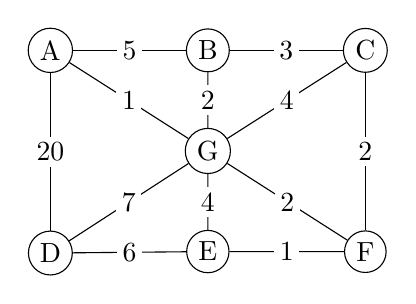
\begin{tikzpicture}
\tikzstyle{vtx}=[draw, circle, inner sep = 2 pt, node distance=2cm]
\tikzstyle{lbl}=[midway, inner sep = 2 pt, fill = white]

\node[vtx] (A)  {A};
\node[vtx, right of =  A] (B) {B};
\node[vtx, right of = B] (C) {C};
\node[vtx, below  = \rr of  B] (E) {E};
\node[vtx, below  = \rr of C] (F) {F};
\node[vtx] (G) at ($(B)!.5!(E)$) {G};
\node[vtx, below = \rr of A] (D) {D};
\foreach \i/\j/\k in {A/B/5, B/C/3, C/F/2,B/G/2,A/D/20, A/G/1, G/E/4, D/E/6, G/F/2,E/F/1, D/G/7, G/C/4}{\draw (\i) -- node[lbl]{\k} (\j);}
\end{tikzpicture}
\end{adjustbox}
%%%
\hfill
%%%%%%%%
\begin{adjustbox}{valign=t,minipage={.4\textwidth}}
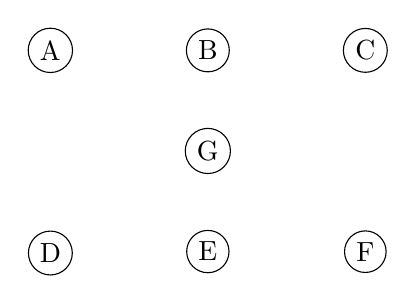
\begin{tikzpicture}
\tikzstyle{vtx}=[draw, circle, inner sep = 2 pt, node distance=2cm]
\tikzstyle{lbl}=[midway, inner sep = 2 pt, fill = white]

\node[vtx] (A)  {A};
\node[vtx, right of =  A] (B) {B};
\node[vtx, right of = B] (C) {C};
\node[vtx, below  = \rr of  B] (E) {E};
\node[vtx, below  = \rr of C] (F) {F};
\node[vtx] (G) at ($(B)!.5!(E)$) {G};
\node[vtx, below = \rr of A] (D) {D};
\end{tikzpicture}
\end{adjustbox}

\vspace{1cm}

\begin{adjustbox}{valign=t,minipage={.1\linewidth}}

{
\renewcommand{\arraystretch}{1.2} 
\begin{tabular}{ c | c | p{.75in}}
Sorted edges & weight & used? \\ \hline
$AG$ & 1 &\\ \hline
$EF$ & 1 &\\ \hline
$BG$ & 2 &\\ \hline
$CF$ & 2&\\ \hline
$FG$ & 2&\\ \hline
$BC$ & 3&\\ \hline
$CG$ & 4 & \\ \hline
$EG$ & 4 &\\ \hline
$AB$ & 5 &\\  \hline
$DE$ & 6&\\ \hline
$DG$ & 7 & \\ \hline
$AD$ & 20&\\ \hline
 \end{tabular}
 }
 \end{adjustbox}
 \hfill
 
\vspace{1cm}

 
\item What is the total cost of the spanning tree you found? \ans
 
\end{subproblems}

\newpage
% page 3 %

%%%
%Cheapest link
%%%
\problem{14 points} 
Recall:

\bigskip

\fbox{Sorted Edges / Cheapest Link Algorithm:}  Select the cheapest edge in the graph that does not create a vertex of degree 3 or close the circuit too soon.

\begin{subproblems}
\item Use \emph{Sorted Edges / Cheapest Link Algorithm} to find a \emph{Hamiltonian circuit} in the following graph. 

Break any ties by choosing the edge that comes earlier in the alphabet. (For example, edge $DC$ is the same edge as edge $CD$, and $CD$ alphabetizes earlier than $GH$.)

Keep track of the cycle in the second graph.

For convenience, the edges of the graph are listed in order in the table below.

\bigskip

\def\rr{2.8}

\begin{adjustbox}{valign=t,minipage={.4\textwidth}}
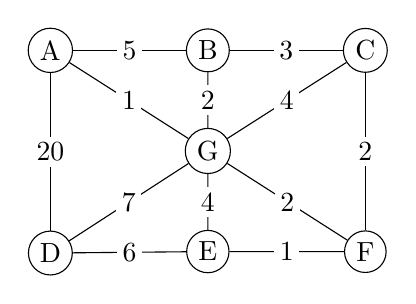
\begin{tikzpicture}
\tikzstyle{vtx}=[draw, circle, inner sep = 2 pt, node distance=2cm]
\tikzstyle{lbl}=[midway, inner sep = 2 pt, fill = white]

\node[vtx] (A)  {A};
\node[vtx, right of =  A] (B) {B};
\node[vtx, right of = B] (C) {C};
\node[vtx, below  = \rr of  B] (E) {E};
\node[vtx, below  = \rr of C] (F) {F};
\node[vtx] (G) at ($(B)!.5!(E)$) {G};
\node[vtx, below = \rr of A] (D) {D};
\foreach \i/\j/\k in {A/B/5, B/C/3, C/F/2,B/G/2,A/D/20, A/G/1, G/E/4, D/E/6, G/F/2,E/F/1, D/G/7, G/C/4}{\draw (\i) -- node[lbl]{\k} (\j);}
\end{tikzpicture}
\end{adjustbox}
%%%
\hfill
%%%%%%%%
\begin{adjustbox}{valign=t,minipage={.4\textwidth}}
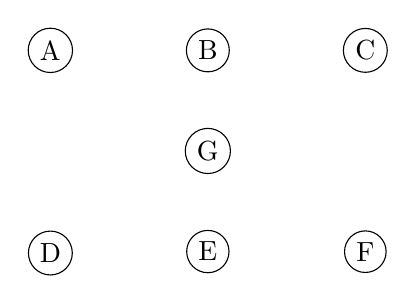
\begin{tikzpicture}
\tikzstyle{vtx}=[draw, circle, inner sep = 2 pt, node distance=2cm]
\tikzstyle{lbl}=[midway, inner sep = 2 pt, fill = white]

\node[vtx] (A)  {A};
\node[vtx, right of =  A] (B) {B};
\node[vtx, right of = B] (C) {C};
\node[vtx, below  = \rr of  B] (E) {E};
\node[vtx, below  = \rr of C] (F) {F};
\node[vtx] (G) at ($(B)!.5!(E)$) {G};
\node[vtx, below = \rr of A] (D) {D};
\end{tikzpicture}
\end{adjustbox}

\bigskip

\begin{adjustbox}{valign=t,minipage={.1\linewidth}}

{
\renewcommand{\arraystretch}{1} 
\begin{tabular}{ c | c | c}
Sorted edges & weight & used? \\ \hline
$AG$ & 1 &\\ \hline
$EF$ & 1 &\\ \hline
$BG$ & 2 &\\ \hline
$CF$ & 2&\\ \hline
$FG$ & 2&\\ \hline
$BC$ & 3&\\ \hline
$CG$ & 4 & \\ \hline
$EG$ & 4 &\\ \hline
$AB$ & 5 &\\  \hline
$DE$ & 6&\\ \hline
$DG$ & 7 & \\ \hline
$AD$ & 20&\\ \hline
 \end{tabular}
 }

 \end{adjustbox}
 %%%%%%
 \hfill
 \vspace{1cm}
 
\item Write the Hamiltonian circuit you found, beginning with vertex $A$. 

\hrulefill

\item What is the total weight of the Hamiltonian circuit? \ans

\item Is this the cheapest possible Hamiltonian circuit in this graph? \ans \  Explain your answer below.
\vfill
 
\end{subproblems}

\newpage
%page 5%

%%%
% scheduling constuction 
%%%
\problem{14 points} 

\def\r{1}
\def\s{.9}

\newcommand{\anotherdigraph}{\begin{tikzpicture}[vtx/.style={draw, circle, inner sep = 3pt, %font = \scriptsize
}, myto/.style={-latex, shorten >=2pt, shorten <=2pt
}, node distance = \r cm]
\node[vtx, label=above:{$A(10)$}, ] (A) at (0,0){};
\node[vtx, below = \s cm of A, label=above:{ $B(5)$}] (B) {};
\node[vtx, below =\s cm of B, label=above:{ $F(3)$}] (F) {};
\node[vtx, right = of B, label=above:{ $C(4)$}] (C) {};
\node[vtx, right = 2*\r of C, label=right:{ $D(1)$}] (D) {};
\node[vtx, below =\s of D, label= right:{ $E(8)$}] (E) {};
\foreach \i/\j in {B/C,F/C,C/D,C/E}{\draw[myto] (\i) -- (\j);}
\draw[myto] (A) to[bend left = 20] (D);

\end{tikzpicture}
}

Consider the following digraph. The units for the tasks are hours.
\begin{center}
\begin{adjustbox}{valign=t,minipage={.4\textwidth}}
\anotherdigraph \hspace{1cm} 
\end{adjustbox}
\begin{adjustbox}{valign=t,minipage={.4\textwidth}}
\begin{tabular}{c | p{1in} | p{1in}}
time & ready & done \\ \hline
&&\\&&\\&&\\&&\\&&\\&&\\&&\\
\end{tabular}
\end{adjustbox}

\end{center}
\begin{subproblems}

\item Construct a schedule for two processors corresponding to the following digraph, given the priority list
\[ B,\;C,\;D,\;F,\; A,\; E\]

Make sure to label the tasks in the schedule. You may use the table to the right of the digraph to track your work.

\begin{center}
\hspace{-1cm}
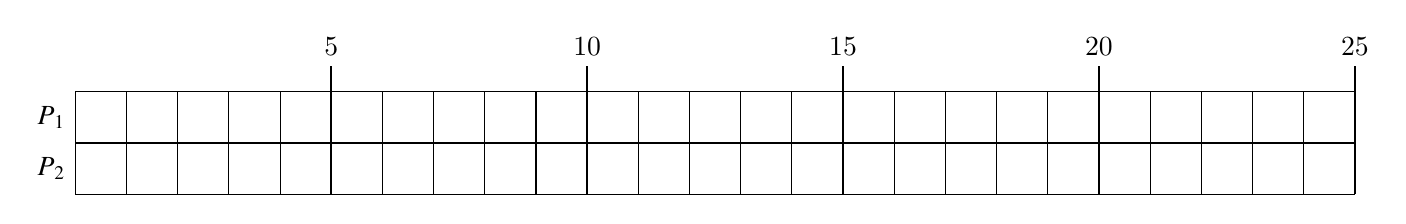
\begin{tikzpicture}[scale = 1.3, lbl/.style={font=\tiny, inner sep = 1 pt, fill = white}]
\path (0, 3/4) node[left] {$P_{1}$};
\path (0, 1/4) node[left] {$P_{2}$};
\draw[step=1/2] (0,0) grid (25/2, 2/2);
\foreach \i in {5, 10, ..., 25}{\draw[thick] (\i/2,0) -- (\i/2,2/2+1/4) node[above]{\i};}
\end{tikzpicture} 
\end{center}

\bigskip

\item How much idle time is in this schedule, and when? \hrulefill

\item How long did this schedule take to complete? \ans

\item What is the critical path and the critical time for this digraph?

\bigskip

Critical path \hrulefill Critical time \ans

\item Is the schedule you found above optimal? Explain your answer: how do you know?

\vfill
\end{subproblems}

\newpage
% page 6 %

%%%
% priority lists, backflow
%%%
\problem{10 points} Consider the following digraph:
\vspace*{-.3in}
\begin{center}
\anotherdigraph
\end{center}

\begin{subproblems}

\item Construct the priority list for the digraph corresponding to the \emph{ decreasing time algorithm. } \\ 

\hrulefill

\item Label the vertices of the digraph according to the \emph{backflow algorithm.}

\item Construct the {priority list} for the digraph corresponding to the \emph{critical path algorithm}. \\

\hrulefill
		
\end{subproblems}

%%%
%Eulerization
%%%
\problem{12 points}
\begin{minipage}{12cm}
	\textbf{a.}  Explain why the graph on the right does not contain an Euler circuit.\\
	
	\vspace{1 in}
	
	\textbf{b.} Eulerize the graph on the right \emph{using as few edge duplications as possible.} Make your added edges very clear!	\\
\end{minipage}
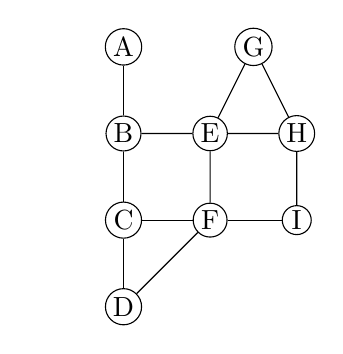
\begin{tikzpicture}[baseline=(current bounding box.center),lbl/.style={inner sep = 1pt, fill = white}, scale = 1.1]
\tikzstyle{vtx}=[circle, draw, inner sep=1pt]
\node at (-1,0){};
\node[vtx] (a) at (0,2) {A};
\node[vtx] (b) at (0,1) {B};
\node[vtx] (c) at (0,0){C};
\node[vtx] (d) at (0,-1){D};
\node[vtx] (e) at (1,1){E};
\node[vtx] (f) at (1,0){F};
\node[vtx] (g) at (1.5,2){G};
\node[vtx] (h) at (2,1){H};
\node[vtx] (i) at (2,0){I};
\foreach \i/\j in {a/b,b/c,c/d,d/f,f/e,e/g,g/h,h/i,i/f,b/e,c/f,e/h}{\draw (\i) -- (\j);}
\end{tikzpicture}

\vfill

\begin{minipage}{12cm}
\textbf{c.} Find an \emph{Euler circuit} in the eulerized graph by \textbf{drawing} the circuit on the (larger) graph to the right and \textbf{listing} the vertices of the circuit in the blank below. (You will have to add your edges from part b in again!)\\
\vspace{.2in}

Euler circuit:  \hrulefill
\end{minipage}
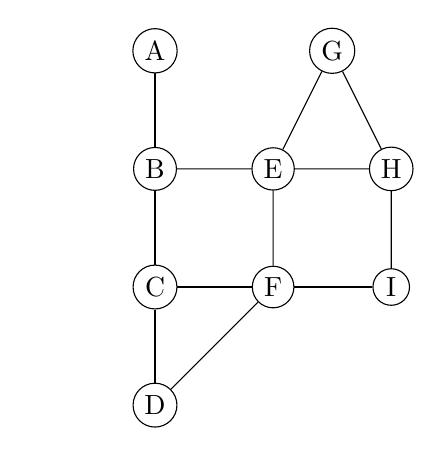
\begin{tikzpicture}[baseline=(current bounding box.center),lbl/.style={inner sep = 2pt, fill = white}, scale = 1.5]
\tikzstyle{vtx}=[circle, draw, inner sep=2pt]
\node at (-1,0){};
\node[vtx] (a) at (0,2) {A};
\node[vtx] (b) at (0,1) {B};
\node[vtx] (c) at (0,0){C};
\node[vtx] (d) at (0,-1){D};
\node[vtx] (e) at (1,1){E};
\node[vtx] (f) at (1,0){F};
\node[vtx] (g) at (1.5,2){G};
\node[vtx] (h) at (2,1){H};
\node[vtx] (i) at (2,0){I};
\foreach \i/\j in {a/b,b/c,c/d,d/f,f/e,e/g,g/h,h/i,i/f,b/e,c/f,e/h}{\draw (\i) -- (\j);}
\end{tikzpicture}
\newpage
%Page 7%

%%%%
% Dijkstra's Algorithm
%%%%
\problem{12 points} Recall Dijkstra's algorithm says the following:

\bigskip
	
	\fbox{Dijkstra's Algorithm}

\textbf{input:} a graph with distances (weights) on the edges and a starting vertex, say $s$\\
\textbf{output:} the shortest distance between $s$ and every vertex in the graph\\
\textbf{rough strategy:} All vertices get \emph{tentative} distances to vertex $s$. One-by-one, vertices are explored and tentative distances are updated until minimum distances are obtained. Break ties alphabetically.\\
	
	\begin{subproblems}
	
\item Use Dijkstra's algorithm to determine the distances between vertex $S$ and each other vertex. Clearly show the steps of the algorithm in the space provided.
	
	\def\ss{6}
\begin{center}
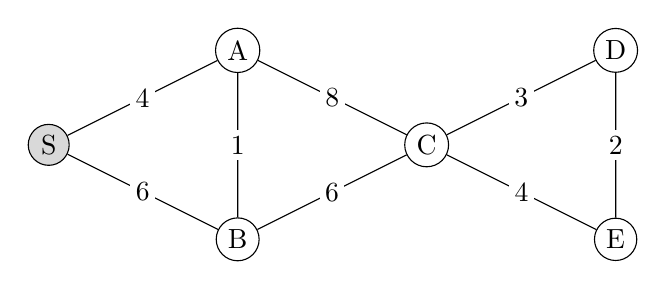
\begin{tikzpicture}[baseline=(current bounding box.center),lbl/.style={inner sep = 2pt, fill = white}, scale = 1.2]
\tikzstyle{vtx}=[circle, draw, inner sep=2pt]
\node[vtx, fill = gray!30] (s) at (0,1) {S};
\node[vtx] (a) at (2,2) {A};
\node[vtx] (b) at (2,0) {B};
\node[vtx] (c) at (4,1){C};
\node[vtx] (d) at (6,2){D};
\node[vtx] (e) at (6,0){E};
\foreach \i/\j/\k in {s/a/4,s/b/6,a/b/1,a/c/8,b/c/6,c/d/3,c/e/4,d/e/2}{\draw (\i) --node[lbl]{\k} (\j);}
\end{tikzpicture}
\end{center}
\begin{minipage}[t]{.6\linewidth}
\begin{tabular}{ c | c | p{1.5in}}
Explored? & vertices & tentative distances\\ \hline
&S& \\[\ss pt] \hline
&A& \\[\ss pt]\hline
&B& \\[\ss pt]\hline
&C& \\[\ss pt]\hline
&D& \\[\ss pt]\hline
&E& \\[\ss pt]\hline
 \end{tabular}

 \end{minipage}
% 
\vspace{1cm}
%
%
 \begin{minipage}{.4\linewidth}
 \begin{tabular}{ c |c }
 vertex & minimum distance to S\\ \hline
S& \\[\ss pt] \hline
A& \\[\ss pt]\hline
B& \\[\ss pt]\hline
C& \\[\ss pt]\hline
D& \\[\ss pt]\hline
E& \\[\ss pt]\hline \end{tabular}
 \end{minipage}
 
 	
\item Which vertex is farthest away from $S$? \ans\  How far is it? \ans
\vfill

\end{subproblems}

\newpage
% page 8 %

%%%%
%Give real world examples
%%%%
 \problem{8 points} Give an example of a real world situation in which you would want to find:
 
 	\begin{subproblems}
	\item a minimum weight Hamiltonian circuit.
	
	\vspace{1in}
	
	\item an Euler circuit.	
	
	\vspace{1in}
	\end{subproblems}
%Extra Credit %
\problem{Extra Credit: 5 points} 
For each of the following, circle the correct answer. Write a few words to justify your answer.

\begin{enumerate}[{True}  $\quad$ {False} $\quad$ (a)]
\item Given any connected finite graph with weighted edges, you can always find an optimal Hamiltonian circuit in a reasonable amount of time.
\vfill
\item Given any graph where the degree of each vertex is even, you can always find an Euler circuit in a reasonable amount of time.
\vfill
\item Given any connected graph, you can always find a minimal-weight spanning tree.
\vfill
\item The critical path algorithm always produces an optimal schedule.
\vfill
\item Adding more processors will always give you a shorter schedule.
\vfill
\end{enumerate}

\end{document}

%%%%ENDDOCUMENT


